\chapter{MiCS Design}

	\section{The MixedSide Principle} % (fold)
	\label{sub:the_mixedside_principle}
		The MixedSide Principle is a constraint that the user has to adhere to in order for MiCS to function correctly. As explained earlier the user can write server side code, which is only meant to be run only on the server, mixed side code, which is meant to be run both on server and client side and client side code, which is only meant to be run client side. The MixedSide Principle describes a simple ruleset for the interaction between serverside, mixedside and clientside code.

		\begin{figure}[H]
			\begin{center}
				\centerline{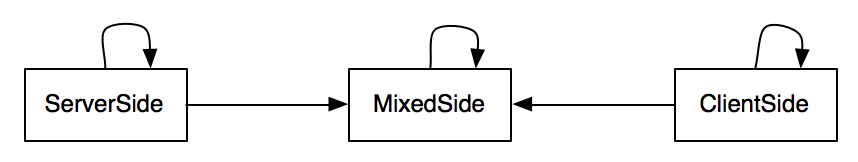
\includegraphics[width=12cm]{resources/images/MixedSidePrinciple.png}}
			\end{center}
			\caption{Visualization of The MixedSide Principle}
			\label{fig:MixedSidePrinciple}
		\end{figure}

		Code annotated with the ClientSide attribute is only meant to be run on the client in form of generated JavaScript. Therefore, it should not make instances of, or calls to methods on, objects that exist only on serverside, as no JavaScript will be generated from server side code. Consequently, if client side code interacts with server side code, it will ultimately result in an error when the JavaScript is generated as some methods and classes will not have been generated. However, JavaScript will be generated from code annotated with either the ClientSide attribute or the MixedSide attribute, so calls from client side to client side or client side to mixed side code are perfectly legal.

		Code that is not annotated with any attributes is regarded as server side code. No JavaScript will be generated from server side code, so server side code should only make calls to other server side code, or to mixed side code.

		As shown in Figure~\ref{fig:MixedSidePrinciple}, MixedSide code should be available both to client side code and server side code. As no communication should happen between client side and server side code, code annotated with the MixedSide attribute should only be able to interact with other code that has also been annotated with the MixedSide attribute. 

		If the MixedSide Principle is not violated and only supported .NET types and members are used, the users’ code is valid.

	% subsection the_mixedside_principle (end)

\section{Workflow Overview} % (fold)
\label{sec:workflow_overview}

This section provides a brief overview of how MiCS works. Figure \ref{fig:mics_internal_workflow} shows the five stages that MiCS goes through when converting C\# to JavaScript.

Basically, MiCS uses Roslyn to generate an AST representing the user’s C\# code. This AST is validated and mapped to a Script\# AST, that represents JavaScript. From the Script\# AST, JavaScript is generated and finally injected into the user’s WebForm page.

\begin{figure}[H]
	\begin{center}
		\centerline{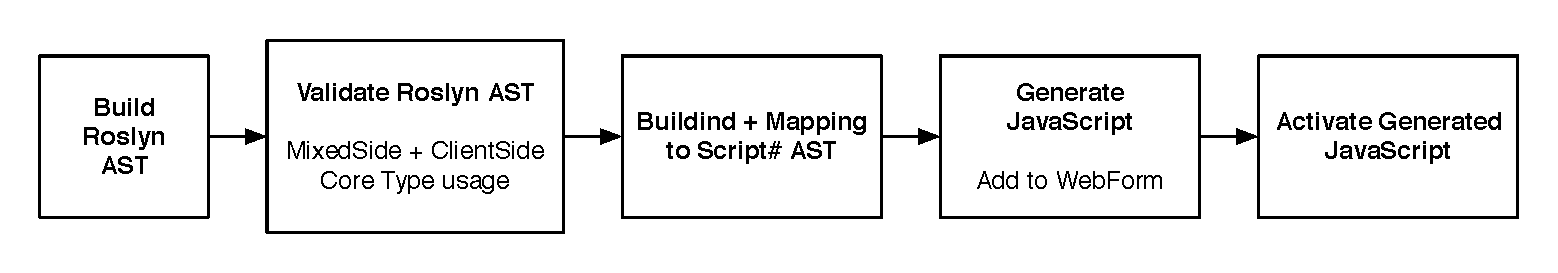
\includegraphics[width=14cm]{resources/images/internalworkflow.eps}}
	\end{center}
	\caption{The MiCS internal workflow}
	\label{fig:mics_internal_workflow}
\end{figure}

MiCS uses Roslyn to generate an Abstract Syntax Tree which is a syntatic representation of the user’s C\# code. Apart from the AST, a Semantic Model is generated to obtain information about what is being referenced.

When the Roslyn AST has been obtained it needs to be validated. This is done to ensure that the user uses types in a correct manner. Without validation, it would be possible for the user to generate non-working JavaScript.

Once the syntax tree has been validated, it is ready to be mapped to Script\#. This is the core functionality of MiCS - transforming a Roslyn AST to a Script\# AST. This step also ensures that the user does not utilize C\# constructs (declarations, statements and expressions) that we do not support. For example, at the moment the only supported loop-type is the for-loop. So if the user uses a while-loop or a foreach loop, the user gets an error telling them that an unsupported construct has been used.

When the Roslyn AST has successfully been mapped to Script\#, MiCS uses Script\#’s built-in ScriptGenerator to generate the JavaScript corresponding to the user’s original C\# code. 

When the JavaScript has been generated, it needs to be injected into the users WebForm. This is handled by a MiCSPage class; an extension to a WebForm Page. 

% section workflow_overview (end)

\section{Architecture} % (fold)
\label{sec:architecture}
Figure \ref{fig:dependencygraph} shows the most essential parts of the internal MiCS architecture and how the parts depend on each other. 
This section will describe the different parts, how they relate to one another and how the architecture relates to the five stages outlined in section \ref{sec:workflow_overview}. 

\begin{figure}
	\begin{center}
		\centerline{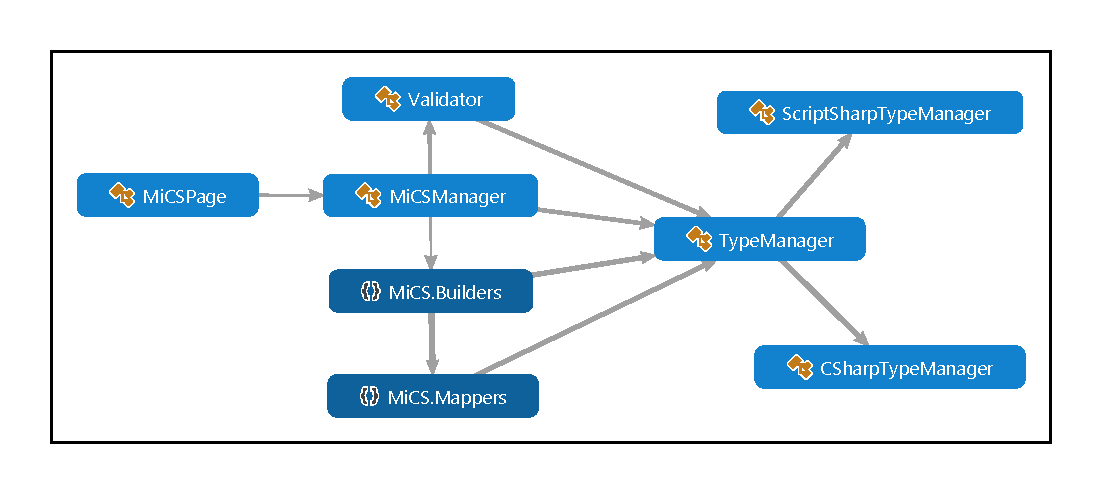
\includegraphics[width=15cm]{resources/images/architecture.pdf}}
	\end{center}
	\caption{The most important parts of the MiCS architecture.}
	\label{fig:dependencygraph}
\end{figure}


The TypeManagers (\texttt{TypeManager}, \texttt{CSharpTypeManager} and\newline \texttt{ScriptSharpTypeManager}) provide information about types used throughout MiCS. For example, the TypeManagers are able to lookup the resultant type of an expression or the type of an identifier (using the Semantic Model described in section \ref{sub:microsoft_roslyn}). Furthermore, they can determine whether a given type is one that the user has defined, or if it is a built-in .NET-type.

The \texttt{Validator} class is responsible for validating the user's code in order to ensure correct type usage before the conversion to Script\# AST begins. The \texttt{Validator} is initiated by the MiCSManager and is dependent on the type managers.

Classes in the Builders and Mappers namespaces are responsible for converting a Roslyn AST to its' corresponding Script\# AST. The Builders traverse the Roslyn AST and build a corresponding Script\# AST. The Builders are dependent on the Mappers which handle the actual conversion from Roslyn SyntaxNodes (AST nodes) to the corresponding Script\# constructs. (Stage 3)

The \texttt{MiCSManager} class ties the entire MiCS project together and is involved in all of the stages described in section \ref{sec:workflow_overview}. It initializes the TypeManagers, starts the validation, and subsequently initiates all of the processes needed to generate JavaScript. 

TODO: Vis og beskriv hvilken del af ScriptSharp vi erstatter med MiCS og Roslyn.
TODO: Update dependency graph

% % section architecture (end)


\section{Detailed Scope}